\section{Experiments and Results}
\label{sec:locvqallm_results}

\subsection{Datasets} 
To evaluate our method, we make use of several publically available datasets: (1) DME-VQA: contains questions on \gls{dme} risk grade and about the presence of biomarkers in the entire image or specific regions. (2) RIS-VQA: contains images from the DaVinci robot during gastrointestinal surgery and questions related to surgical instruments. (3) INSEGCAT-VQA: contains frames from cataract surgery videos and questions about instruments used in this type of surgery. A summary of these is shown in Table~\ref{tab:locvqallm_datasets}, based on~\cite{tascon2023localized}.

\begin{table}[ht]
\begin{center}
\begin{tabular}{lp{0.5cm}lp{0.5cm}cp{0.5cm}c}
\toprule
Dataset                       && Modality         && \# images && \# QA-pairs \\ \midrule
DME-VQA                        && Fundus && 679 && 13470 \\
RIS-VQA                        && Gastrointestinal && 2978 && 32562 \\
INSEGCAT-VQA                   && Cataract surgery && 4647 && 39008 \\
\bottomrule
\end{tabular}
\end{center}
\caption{Main parameters of the used datasets.}
\label{tab:locvqallm_datasets}
\end{table}

\subsection{Baselines} 
We benchmark our method against multiple baselines, which are exemplified in Fig.~\ref{fig:locvqallm_baselines}. In \textbf{No mask}, the model receives no information about the location of the region; in \textbf{Region in text}, the region is specified in the question; in \textbf{Draw region}, the region is marked on top of the image. In \textbf{Context only}, the model only sees the context, but not the contents of the region; in \textbf{Crop region}, the model receives no context; finally, in \textbf{LocAtt}~\cite{tascon2023localized}, the model has access to the image, as well as a binary image representing the region. For these baselines, the visual prompt given to the model is: \textit{``Answer the question below using the context below Context: $<$Img$><$Image$><$/Img$>$Question:$<$Question$>$Answer:"}
\begin{figure}[b]
\begin{center}
\includegraphics[width=\textwidth]{Figures/Part1_LocVQA/02_llm/baselines.pdf}
\caption{Example input images and questions for evaluated baselines. In the baseline ``Region in text," the digits are separated to provide a fair scenario to the LLM.}
\label{fig:locvqallm_baselines}
\end{center}
\end{figure}

\subsection{Implementation Details} 
We use R2GenGPT~\cite{wang2023r2gengpt} as base \gls{mllm}, adapting it from the task of radiology report generation to \gls{vqa}. Following the original implementation of R2GenGPT, we use a pre-trained Swin Transformer~\cite{liu2021swin} as a visual encoder and Llama 2~\cite{touvron2023llama} as \gls{llm} initialized with its official weights. Different from to R2GenGPT, we finetune all modules, including the \gls{llm}, end-to-end. We use the default parameters for the selected backbone model: We train all our models for 15 epochs, with a batch size of 8 and a learning rate of 1e-4, with the AdamW optimizer and a cosine annealing scheduler with a minimum learning rate of 1e-6. For the text generation, we use a repetition penalty of 2.0 as in~\cite{wang2023r2gengpt} but establish a length penalty of -1.0 to encourage short answers. Our implementation uses PyTorch 2.0.1 and two Nvidia A100 cards with 80 GB of memory each.

\subsection{Results} 
\label{sec:locvqallm_results}

Table~\ref{tab:locvqallm_results} summarizes our results on the DME-VQA, RIS-VQA, and INSEGCAT-VQA datasets. The accuracy and F1 score are reported for all datasets. Notably, our method consistently outperforms all evaluated baselines across all datasets, underscoring the efficacy of targeted visual prompting in enhancing \glspl{mllm} with region-based capabilities. 

\begin{table}[!t]
\begin{center}
\begin{tabular}{lp{0.5cm}lp{0.5cm}cp{0.5cm}cp{0.5cm}}
\toprule
Dataset                       && Method         && Accuracy (\%) && F1 score (\%) \\ \midrule
\multirow{7}{*}{DME-VQA}      && No Mask    && 57.32 &&    57.32   \\ 
                                && Region in Text~\cite{vu2020question} &&  62.12 &&  63.59 \\ 
                              && Crop Region~\cite{tascon2022consistency}    &&  86.52   &&  87.26   \\ 
                              %&& Adapted LocAtt~\cite{tascon2023localized}$^\dag$  && 86.30 \\
                              && Draw Region && 86.86 && 86.85 \\ 
                              && Context Only && 88.07  && 88.45 \\ 
                              && \ours           && \textbf{90.30} && \textbf{90.22} \\ 
                             && \textcolor{gray}{LocAtt~\cite{tascon2023localized}$^*$}  && \textcolor{gray}{84.2} && \textcolor{gray}{85.79}  \\
\midrule
\multirow{7}{*}{RIS-VQA}      && No Mask    && 50.00  &&  50.00   \\ 
                                && Region in Text~\cite{vu2020question} &&  64.81 &&  65.39\\ 
                              && Crop Region~\cite{tascon2022consistency}    &&  85.50  &&   85.64   \\ 
                              %&& Adapted LocAtt~\cite{tascon2023localized}$^\dag$  && 86.30 \\
                              && Draw Region && 91.30  && 91.43 \\ 
                              && Context Only && 91.77 && 91.81  \\ 
                              && \ours           && \textbf{92.60} && \textbf{92.54} \\ 
                             && \textcolor{gray}{LocAtt~\cite{tascon2023localized}$^*$}  && \textcolor{gray}{82.73} &&  \textcolor{gray}{86.15}\\
                              \midrule
\multirow{7}{*}{INSEGCAT-VQA} && No Mask    &&   50.00  &&  50.00  \\  
                              && Region in Text~\cite{vu2020question} &&  73.51  && 74.55 \\ 
                              && Crop Region~\cite{tascon2022consistency}    &&  90.91  &&  90.93  \\ 
                              %&& Adapted LocAtt~\cite{tascon2023localized}$^\dag$  && 89.89 \\
                              && Draw Region && 95.44 && 95.43\\  
                            && Context Only && 95.19 &&  95.17 \\ 
                              && \ours           &&  \textbf{95.51}    &&  \textbf{95.47} \\
                              && \textcolor{gray}{LocAtt~\cite{tascon2023localized}$^*$}  && \textcolor{gray}{88.13} && \textcolor{gray}{90.14}\\                              
                              \bottomrule
\end{tabular}
\end{center}
\caption{Accuracy and F1 score comparison to SOTA approaches on the DME-VQA, RIS-VQA and INSEGCAT-VQA datasets. For the DME-VQA dataset, only localized questions are considered (performance on other question types can be found in the supplementary materials). $^*$This result corresponds to a different architecture, but we include it for completeness. }
\label{tab:locvqallm_results}
\end{table}

In the case of the DME-VQA and RIS-VQA datasets, we observe that the performance of \textit{context only} surpasses that of \textit{crop region}. At first glance, this suggests that the context holds more relevance than the specific contents of the region. However, this behavior is likely influenced by spurious correlations between region sizes, locations, and the corresponding answers. For instance, in DME-VQA, images with a high amount of biomarkers often feature smaller regions associated with negative answers. Similarly, in RIS-VQA, the tool can often be determined from its body without considering the tip. 

Notably, the \textit{region in text} baseline exhibits poor performance. Given the use of a powerful \gls{llm} in the pipeline, higher performance might be expected. Different variations were explored for this baseline, including not separating the coordinate digits or replacing coordinate digits with words, but performance did not improve. We hypothesize that the model fails to correctly map location information from the text to the image, which can be at least partly attributed to using a \gls{vit} to embed the image.

We provide qualitative example results in Fig.~\ref{fig:locvqallm_examples}. The first column exemplifies cases where our method demonstrates robustness to subtle evidence (small biomarkers), correlations (surgical suture is usually close to the needle driver), and borderline cases (evidence close to the region). The second column highlights the weaknesses of \textit{context only} when the context fails to provide enough evidence for the answer. Finally, the third column shows errors made by our model.
\begin{figure}[!t]
\begin{center}
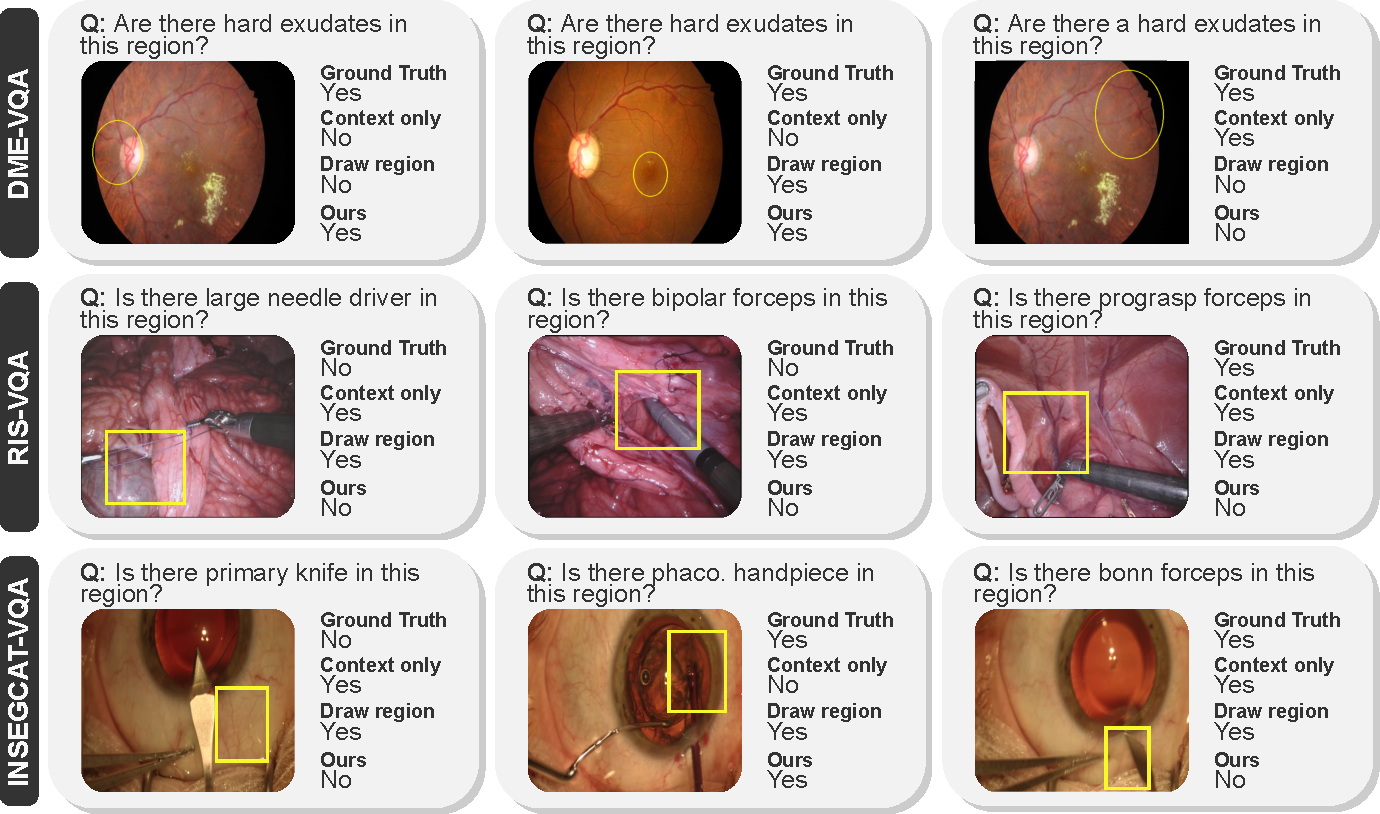
\includegraphics[width=0.90\textwidth]{Figures/Part1_LocVQA/02_llm/examples.pdf}
\caption{Qualitative examples on the DME-VQA (first row), RIS-VQA (second row), and INSEGCAT-VQA (third row) datasets. See Appendix~\ref{appendix:locvqallm} for additional examples.}
\label{fig:locvqallm_examples}
\end{center}
\end{figure}
Fig.~\ref{fig:locvqallm_errors_by_location} shows error maps by region location for the DME-VQA and INSEGCAT-VQA datasets and for the four strongest baselines. On the left side of the plot, the locations of actual positives and negatives are illustrated. For the INSEGCAT-VQA dataset, this visualization reveals a location bias that other baselines without access to the region or the context may be exploiting. Due to the nature of the images (cataract surgery) and questions, regions with positive answers tend to cluster in a specific area. This, coupled with the dissimilarity of objects mentioned in the questions, explains why a baseline like \textit{crop region} achieves relatively high performance on this dataset compared to the other two datasets (see Table~\ref{tab:locvqallm_results}). Similarly, in the case of DME-VQA, it becomes evident that the lack of context in \textit{crop region} results in lower sensitivity, highlighting the significance of context even when the isolated region should theoretically provide sufficient evidence. Fig.~\ref{fig:locvqallm_errors_by_location} also demonstrates that \textit{draw region} and \textit{context only} exhibit marked clusters of false positives and false negatives, potentially indicating the utilization of location biases. In contrast, our method produces a more evenly distributed location for both types of errors.
\begin{figure}[!b]
\begin{center}
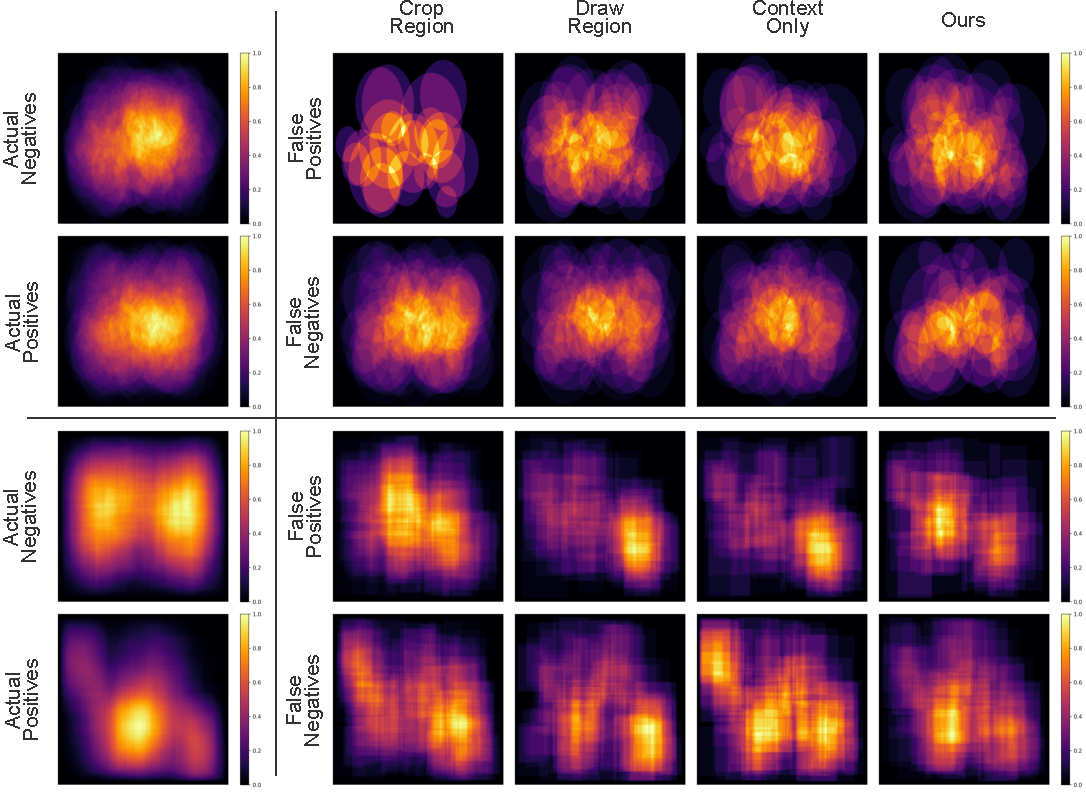
\includegraphics[width=0.85\textwidth]{Figures/Part1_LocVQA/02_llm/errors_by_location.pdf}
\caption{Error analysis by region location for the four strongest baselines. The maps are obtained by adding binary masks representing the regions for all QA pairs in each category and then normalizing. \textbf{Top:} DME-VQA dataset. \textbf{Bottom:} INSEGCAT-VQA dataset. The maps for RIS-VQA can be found in Appendix~\ref{appendix:locvqallm}.}
\label{fig:locvqallm_errors_by_location}
\end{center}
\end{figure}


